% !TEX root = ../thesis.tex

%%%%%%%%%%%%%%%%%%%%%%%%%%%%%%%%%%%%%%%%%%%%%%%%%%%%%%%%%%%
% Chapter: Example Application
%%%%%%%%%%%%%%%%%%%%%%%%%%%%%%%%%%%%%%%%%%%%%%%%%%%%%%%%%%%
\chapter{Example Application: State Machine}\label{Example Application}
In this chapter in order to show how our managed data implementation works in practice, and in particular in terms of aspect refactoring, we present a showcase.
The showcase consists of a very simple state machine application.
A similar example is presented in Enso paper as a showcase for its Object Grammar capabilities \cite{storm2012object}.

Consider the requirements of the state machine as the following: 
\begin{itemize}
	\item A state \texttt{Machine} consists of a number of named \texttt{State} declarations.

	\item Each \texttt{State} contains \texttt{Transitions} to other states, which are identified by a \texttt{name}, when a certain event happens.

	\item A \texttt{Transition} is identified by a certain \texttt{event}.
\end{itemize}

For reasons of simplicity, this example will be a very basic \textit{door} state machine, which includes three states \textbf{Open}, \textbf{Close} and \textbf{Locked}, accompanied by their transitions: \textbf{open\_door}, \textbf{close\_door}, \textbf{lock\_door} and \textbf{unlock\_door} respectively.
Figure \ref{fig:State_machine} illustrates the door state machine.

\begin{figure}[H]
	\centering
  	\fbox{\includegraphics[width=.40\textwidth]{figures/State_machine.png}}
  	\caption{Basic door state machine}
  	\label{fig:State_machine}
\end{figure}

To implement this we need to define the models, interpret the definition given from a list of events and finally add any additional functionality (\textit{concern}) needed, in our case we will implement logging of door's current state.

%%%%%%%%%%%%%%%%%%%%%%%%%%%%%%%%%%%%%%%%%%%%%%%%%%%%%%%%%%%%%
\section{Schemas definition}
As a first step, all the models of the state machine program need to be defined. 
An object diagram is illustrated in Figure \ref{fig:State_machine_object}.

\begin{figure}[H]
	\centering
  	\fbox{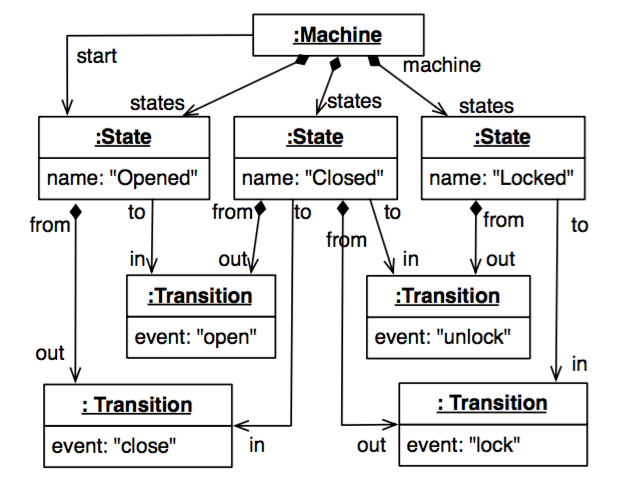
\includegraphics[width=.50\textwidth]{figures/State_machine_object_diagram.png}}
  	\caption{Basic door state machine object diagram}
  	\label{fig:State_machine_object}
\end{figure}

In our implementation we define schemas using Java interfaces with a set of meta-data described with Java annotations.
Therefore, as extracted from the requirements we need \texttt{Machine} (Listing \ref{lst:Machine_Schema}), \texttt{State} (Listing \ref{lst:State_Schema}) and \texttt{Transition} (Listing \ref{lst:Transition_Schema}) schemas.

%%%%%%%%%%%%%%%%%%%%%%%%%%%%%%%%%%%%%%%%%%%%%%%%%%%%%%%%%%%
\begin{sourcecode}[H]
	\begin{lstlisting}[language=Java,escapechar=|]
public interface Machine extends M {
	State start(State... startingState);

	State current(State... currentState);

	@Contain
	Set<State> states(State... states);
}
	\end{lstlisting}
	\caption{The Machine Schema}
	\label{lst:Machine_Schema}
\end{sourcecode}

As it can be seen in Listing \ref{lst:Machine_Schema}, the \texttt{Machine} schema definition requires a \texttt{start}ing state, the \texttt{current} state of the machine and a set of \texttt{states} that the machine can be into at each time.
Note that the \texttt{@Contain} annotation suggests that the \texttt{states} field is part of the spine tree and it is not a cross-reference.
This will be further explained in Chapter \ref{Implementation}.

%%%%%%%%%%%%%%%%%%%%%%%%%%%%%%%%%%%%%%%%%%%%%%%%%%%%%%%%%%%%%%%%%%%%%%%%%%%%%%%
\begin{sourcecode}[H]
	\begin{lstlisting}[language=Java,escapechar=|]
public interface State extends M {
	@Key
	String name(String... name);

	@Inverse(other = Machine.class, field = "states")
	Machine machine(Machine... machine);

	@Contain
	Set<Transition> out(Transition... transition);

	@Contain
	Set<Transition> in(Transition... transition);
}
	\end{lstlisting}
	\caption{The State Schema}
	\label{lst:State_Schema}
\end{sourcecode}

For the \texttt{State} definition, Listing \ref{lst:State_Schema}, we need a \texttt{name} field, which represents the name of the state. 
This \texttt{name} field has been annotated with the \texttt{@Key} annotation, which indicates uniqueness. 
The states field of Machine can be indexed by name.
Moreover, the schema includes a set of \texttt{in} and \texttt{out} \texttt{Transition}s.
Since those two fields are of type \texttt{Set}, one field of the \texttt{Transition} schema has to be marked as \textit{key}.
In this case, it is the \texttt{name} field (Line \ref{line:transition_key} Listing \ref{lst:Transition_Schema}).
Finally, the field \texttt{machine} represents the state machine that the state is part of. 
As it can be seen in the schema definition, Listing \ref{lst:State_Schema}, the \texttt{machine} field has been annotated with \texttt{@Inverse}, which indicates that this field is a reference to a field of another schema.
In this case, the \texttt{machine} field of \texttt{State} schema is a reference to \texttt{states} field of \texttt{Machine} schema.

%%%%%%%%%%%%%%%%%%%%%%%%%%%%%%%%%%%%%%%%%%%%%%%%%%%%%%%
\begin{sourcecode}[H]
	\begin{lstlisting}[language=Java,escapechar=|]
public interface Transition extends M {
	@Key 					|\label{line:transition_key}| 
	String event(String... event);

	@Inverse(other = State.class, field = "out")
	State from(State... from);

	@Inverse(other = State.class, field = "in")
	State to(State... to);
}
	\end{lstlisting}
	\caption{The Transition Schema}
	\label{lst:Transition_Schema}
\end{sourcecode}

Finally, in the \texttt{Transition} schema definition, Listing \ref{lst:Transition_Schema}, we need an \texttt{event} that corresponds to the event of the transition and is the \textbf{key} of that schema.
The \texttt{from} and \texttt{to} fields represent the state that the machine changes from and to respectively.
However, these are just references to the \texttt{State} schema (Listing \ref{lst:State_Schema}).

%%%%%%%%%%%%%%%%%%%%%%%%%%%%%%%%%%%%%%%%%%%%%%%%%%%%%%%
\section{Factory definition}
Now that we have our schemas, we need a way to build instances of managed objects that these schemas describe. 
In Java to create these three schemas as managed data we need to define a factory, which creates managed data instances (managed objects) for each of these schemas \ref{lst:StateMachineFactory}.
Note that the method definitions work as \texttt{Constructors} of managed objects.

\begin{sourcecode}[H]
	\begin{lstlisting}[language=Java,escapechar=|]
public interface StateMachineFactory extends IFactory {
	Machine Machine();  		// constructor for Machine managed objects
	State State(); 				// constructor for State managed objects
	Transition Transition(); 	// constructor for Transition managed objects
}
	\end{lstlisting}
	\caption{The StateMachine Factory}
	\label{lst:StateMachineFactory}
\end{sourcecode}

%%%%%%%%%%%%%%%%%%%%%%%%%%%%%%%%%%%%%%%%%%%%%%%%%%%%%%%
\section{Basic Data Manager}
As mentioned above, in order to interpret and manage the defined data we need data managers. 
Our implementation includes the definition of a \texttt{Basic data manager} that is responsible of interpreting a schema definition to instances of \textit{managed object}s.
Conclusively, in order to make a \textit{managed object}, the data manager needs its schema definition (the interfaces that define the schemas) and the factory (the interface that defines the constructors of the schemas).

%%%%%%%%%%%%%%%%%%%%%%%%%%%%%%%%%%%%%%%%%%%%%%%%%%%%%%%
\subsection{A simple program}
In the case of a simple program without any concerns, we have to use our managed data to define the state machine and then interpret it.
The definition of the door state machine is given in Listing \ref{lst:Door_state_machine} in Java.

In practice, the basic data manager needs to provide us with mechanisms that interpret the managed object that based on \texttt{stateMachineSchema}, shown in Line \ref{line:state_meaning_full_code}.
The basic data manager  also supports the field accessors of those data, namely, the setters and getters of their values.
An basic interpreter for the state machine is shown in Line \ref{line:state_machine_interpreter}.
As it can be seen, the factory is used to create managed objects.
The \textit{setup} of the fields is done automatically by the data manager who is responsible for the managed object interpretation.

\begin{sourcecode}
	\begin{lstlisting}[language=Java, escapechar=|]
public class StateMachineExample {
	public static void main(String[] args) {
		SchemaFactory schemaFactory = ...;
		Schema stateMachineSchema = SchemaLoader
			.load(schemaFactory, Machine.class, State.class, Transition.class); |\label{line:state_schemaMachineSchema}|

		BasicDataManager basicDataManager = new BasicDataManager(); |\label{line:state_meaning_full_code}|
		StateMachineFactory stateMachineFactory = 
			basicDataManager.factory(StateMachineFactory.class, stateMachineSchema);

		Machine doorStateMachine = stateMachineFactory.Machine(); |\label{line:state_machine_creation_basic}|

		State openState = stateMachineFactory.State(OPEN_STATE);
		openState.machine(doorStateMachine);

		State closedState = stateMachineFactory.State(CLOSED_STATE);
		closedState.machine(doorStateMachine);

		State lockedState = stateMachineFactory.State(LOCKED_STATE);
		lockedState.machine(doorStateMachine);

		Transition closeTransition = stateMachineFactory.Transition(CLOSE_TRANSITION);
		closeTransition.from(openState); closeTransition.to(closedState);

		Transition openTransition = stateMachineFactory.Transition(OPEN_TRANSITION);
		openTransition.from(closedState); openTransition.to(openState);

		Transition lockTransition = stateMachineFactory.Transition(LOCK_TRANSITION);
		lockTransition.from(closedState); lockTransition.to(lockedState);

		Transition unlockTransition = stateMachineFactory.Transition(UNLOCK_TRANSITION);
		unlockTransition.from(lockedState); unlockTransition.to(closedState);

		doorStateMachine.start(closedState);
		interpretStateMachine(doorStateMachine, new LinkedList<>(Arrays.asList(
				LOCK_TRANSITION,
				UNLOCK_TRANSITION,
				OPEN_TRANSITION)));
		}	
	}

	private static void interpretStateMachine(
			Machine stateMachine, List<String> commands) 
	{ |\label{line:state_machine_interpreter}|
	    stateMachine.current(stateMachine.start());
		for (String event : commands) {
			for (Transition trans : stateMachine.current().out()) {
				if (trans.event().equals(event)) {
					stateMachine.current(trans.to());
					break;
				}
			}
	}
}
	\end{lstlisting}
	\caption{Door state machine}
	\label{lst:Door_state_machine}
\end{sourcecode}

%%%%%%%%%%%%%%%%%%%%%%%%%%%%%%%%%%%%%%%%%%%%%%%%%%%%%%%
%%%%%%%%%%%%%%%%%%%%%%%%%%%%%%%%%%%%%%%%%%%%%%%%%%%%%%%
%%%%%%%%%%%%%%%%%%%%%%%%%%%%%%%%%%%%%%%%%%%%%%%%%%%%%%%
\section{Logging crosscutting concern}
Now consider a case where we want to add a crosscutting concern at the previous door state machine implementation.
A simple concern could be \textit{logging}, which would log every change in the ``current'' state of the door state machine.

In order to implement this concern we need a mechanism that continuously observes the changes (transitions) of the machine's \texttt{current} state and reacts accordingly.
Usually, this would lead to scattered logging code in the interpretation method or the models themselves (the machine model).
This is where data managers come to the rescue.
A data manager can implement concerns as modular aspects without scattering code to the components.
The programmer can define a manipulation mechanism of his/her data that includes an aspect of preference.
Therefore, by implementing our concern with a data manager we can keep the component and aspect code separate.

%%%%%%%%%%%%%%%%%%%%%%%%%%%%%%%%%%%%%%%%%%%%%%%%%%%%%%%
\subsection{Observable Data Manager}
Regarding the continuous \textit{observation} of our state machine's ``current'' state changes, we need a data manager that observes these changes in a managed object and executes actions defined by the programmer.
Particularly, it has to observe the \texttt{Machine}'s current \texttt{State} field and perform logging in case this field's value changes.
This data manager creates concrete managed objects as subjects, where observers can be attached in order to be notified of changes and execute an action.
It is important to mention that this new data manager has to inherit the basic one in order to include the basic functionality of schema interpretation and field access.
This leads to a \textbf{stack} of two data managers, each one adding a new aspect of data in a modular way.

In order to define the specifications of our new data manager we first need to define how it is going to be used (its API).
First, we need to attach the \textit{logging} concern to our \texttt{Machine} object. 
This is going to be executed in case the \texttt{current} state changes.
The client code can be seen in Listing \ref{lst:StateMachineMonitoringConcerns}.

\begin{sourcecode} [H]
	\begin{lstlisting}[language=Java, escapechar=|]
ObservableDataManager observableDataManager = new 	ObservableDataManager();
StateMachineFactory stateChangesMachineFactory =
	observableDataManager.factory(StateMachineFactory.class, stateMachineSchema);

Machine doorStateMachine = stateChangesMachineFactory.Machine();

((Observable) doorStateMachine) // Add logging concern on current field changes
	.observe((obj, fieldName, newState) -> { |\label{line:state_machine_monitor}|
		if (fieldName.equals("current")) {
			System.out.println(" > State changed to " + ((State)newState).name());
		}
	});
	\end{lstlisting}
	\caption{Door state machine with logging concern}
	\label{lst:StateMachineMonitoringConcerns}
\end{sourcecode}

%%%%%%%%%%%%%%%%%%%%%%%%%%%%%%%%%%%%%%%%%%%%%%%%%%%%%%%
\subsection{Data Manager Implementation}
Now that we have specified the API of our data manager, we need to implement it.
First, we need to define our specifications.
As it can be seen from Listing \ref{lst:StateMachineMonitoringConcerns}, the \texttt{ObservableDataManager} provides a managed object with the method \texttt{observe}, which adds observers on field changes.

More specifically, this data manager allows to add observers in managed data in the form of a functional interface.
The observe action is shown in Listing \ref{lst:Observe functional interface}.

\begin{sourcecode} [H]
	\begin{lstlisting}[language=Java, escapechar=|]
@FunctionalInterface
public interface Observe {
	void observe(Object obj, String fieldName, Object newValue);
}
	\end{lstlisting}
	\caption{Observe Functional Interface}
	\label{lst:Observe functional interface}
\end{sourcecode}

This functional interface represents an action that is performed when a field changes.
In order to be executed, an action needs to be added in an list of observers.
This specification can be defined in an interface, shown in Listing \ref{lst:Observable interface}.

\begin{sourcecode} [H]
	\begin{lstlisting}[language=Java, escapechar=|]
public interface Observable {
	void observe(Observe _observer);
}
	\end{lstlisting}
	\caption{Observable Interface}
	\label{lst:Observable interface}
\end{sourcecode}

This interface describes the specification for our data manager.
The proxy factory code is shown in Listing \ref{lst:ObservableDataManager} and its MObject implementation in Listing \ref{lst:ObservableMObject}.

\begin{sourcecode} [H]
	\begin{lstlisting}[language=Java, escapechar=|]
public class ObservableDataManager extends BasicDataManager {

    @Override
    public <T extends IFactory> T factory(
    	Class<T> moSchemaFactoryClass, Schema schema, Class<?>... proxiedInterfaces) 
    {
        return super.factory(moSchemaFactoryClass, schema, Observable.class);
    }

    @Override
    protected MObject createManagedObject(Klass klass, Object... _inits) {
        return new ObservableMObject(klass, _inits);
    }
}
	\end{lstlisting}
	\caption{ObservableDataManager - Proxy factory}
	\label{lst:ObservableDataManager}
\end{sourcecode}

Note that the \texttt{ObservableDataManager} adds the \texttt{Observable.class} in its proxy interfaces.
By doing this, the managed object can be ``casted'' as an \texttt{Observable} and adopt the data manager's functionality, as shown in the client code Listing \ref{lst:StateMachineMonitoringConcerns}.

\begin{sourcecode} [H]
	\begin{lstlisting}[language=Java, escapechar=|]
public class ObservableMObject extends MObject implements Observable {
	// a list of observers for that object
	private List<Observe> observers;

	public ObservableMObject(Klass schemaKlass, Object... initializers) {
		super(schemaKlass, initializers);
		observers = new ArrayList<Observe>();
	}

	public void observe(Observe _observer) {
		observers.add(_observer);
	}

	@Override
	public void _set(String _name, Object _value) {
		super._set(_name, _value);
		// Run the observe function for each of the observers on every "set"
		observers.forEach(observer -> observer.observe(thisObject, _name, _value));
	}
}
	\end{lstlisting}
	\caption{ObservableMObject - Invocation Handler}
	\label{lst:ObservableMObject}
\end{sourcecode}

The data manager keeps a list of \texttt{Observe} actions.
The programmer can add actions by using the \texttt{observe} method.
Every time a field's value changes, calling the \texttt{\_set} method of the \texttt{MObject}, the list of the observer actions is executed.
Note that this data manager is general, it does not exclusively work for \texttt{Machine} objects, as in this case, but for all managed objects.

Concluding, it can be observed that the only part that has been changed in the original code is the data manager and the logging concern definition.
The data manager of the \texttt{Machine} managed object has been changed to the new observable data manager.
Additionally, the logging concern has been attached to the machine object very easily simply by using lambdas (Line \ref{line:state_machine_monitor} of Listing \ref{lst:StateMachineMonitoringConcerns}).

By running the program with the commands \texttt{LOCK\_TRANSITION}, \texttt{UNLOCK\_TRANSITION} and \texttt{OPEN\_TRANSITION}, the output is presented in Listing \ref{lst:StateMachineMonitoringConcernsOutput}.
\lstdefinestyle{Bash} {
    backgroundcolor=\color{white},
    basicstyle=\scriptsize\color{black}\ttfamily
}

\begin{sourcecode} [H]
	\lstset{numbers=none}
	\begin{lstlisting}[style=Bash]
> Current state changed to Closed
> Current state changed to Locked
> Current state changed to Open
	\end{lstlisting}
	\caption{Door state machine with logging concern: output}
	\label{lst:StateMachineMonitoringConcernsOutput}
\end{sourcecode}

The basic data manager allows to solely build managed objects, but the observable data manager also provides the functionality of attaching concerns in the managed objects after a specified event.

%%%%%%%%%%%%%%%%%%%%%%%%%%%%%%%%%%%%%%%%%%%%%%%%%%%%%%%
%%%%%%%%%%%%%%%%%%%%%%%%%%%%%%%%%%%%%%%%%%%%%%%%%%%%%%%
%%%%%%%%%%%%%%%%%%%%%%%%%%%%%%%%%%%%%%%%%%%%%%%%%%%%%%%
\section{Combine crosscutting concern}
One of managed data main characteristics is that it allows to define reusable aspects but also to combine them independently.
The concerns do not know about each other while a new data manager can combine them.
An example of this can be shown in Figure \ref{fig:concerns_combination}.

\begin{figure}[H]
	\centering
  	\fbox{\includegraphics[width=1\textwidth]{figures/Example_Class_Diagram.png}}
  	\caption{Combination of logging and immutability concerns}
  	\label{fig:concerns_combination}
\end{figure}

As the figure shows there are two separate concerns implemented in \texttt{MObjects}, namely \texttt{Observable} and \texttt{Lockable}.
Consider that we want to add the \texttt{Lockable} feature (immutability) in our previous door state machine while the \texttt{Observable} functionality still exists.
The client code for this is presented in Listing \ref{lst:StateMachineMonitoringConcernsCombination}.
The \texttt{Lockable} data manager is presented in detail in Section \ref{Implementing a Data Manager}.

\begin{sourcecode} [H]
	\begin{lstlisting}[language=Java, escapechar=|]
// The new data manger that combines two aspects
LockableObservableDataManager dataManager = new 	LockableObservableDataManager();
StateMachineFactory stateChangesMachineFactory =
	dataManager.factory(StateMachineFactory.class, stateMachineSchema);

final Machine doorStateMachine = stateChangesMachineFactory.Machine();

((Observable) doorStateMachine) // Add logging concern on current field changes
	.observe((obj, fieldName, newState) -> {
		if (fieldName.equals("current")) {
			System.out.println(" > State changed to " + ((State)newState).name());
		}
	});
// ...
// It was mutable until now, will not allow changes from now on.
((Lockable) doorStateMachine).lock(); // Add immutability concern 
// ...
	\end{lstlisting}
	\caption{Door state machine with logging and immutability concerns}
	\label{lst:StateMachineMonitoringConcernsCombination}
\end{sourcecode}

The new \texttt{MObject} simply combines the two aspects by using composition of \texttt{LockableMObject} and \texttt{ObservableMObject} instances.
By overriding the methods defined by the \texttt{Lockable} and \texttt{Observable} interfaces and using the \texttt{LockableMObject} and \texttt{ObservableMObject} instances respectively, the new data manager combines the two concerns in a modular way.
Listings \ref{lst:LockableObservableMObject} and \ref{lst:LockableObservableDataManager} show this implementation.

\begin{sourcecode} [H]
	\begin{lstlisting}[language=Java, escapechar=|]
public class LockableObservableMObject 
	extends MObject implements Lockable, Observable 
	{

	private LockableMObject lockableMObject;
	private ObservableMObject observableMObject;

	public LockableObservableMObject(Klass schemaKlass, Object... initializers) {
		super(schemaKlass, initializers);
		lockableMObject = new LockableMObject(schemaKlass, initializers);
		observableMObject = new ObservableMObject(schemaKlass, initializers);
	}

	@Override
	public void observe(Observe _observer) {
		observableMObject.observe(_observer);
	}

	@Override
	public void lock() {
		lockableMObject.lock();
	}

	@Override
	public void _set(String name, Object value) {
		lockableMObject._set(name, value);
		observableMObject._set(name, value);
		super._set(name, value);
	}
}
	\end{lstlisting}
	\caption{LockableObservableMObject}
	\label{lst:LockableObservableMObject}
\end{sourcecode}

\begin{sourcecode} [H]
	\begin{lstlisting}[language=Java, escapechar=|]
public class LockableObservableDataManager extends BasicDataManager {

	@Override
	public <T extends IFactory> T factory(
		Class<T> factoryClass, Schema schema, Class<?>... additionalInterfaces) 
	{
		return super.factory(factoryClass, schema, Lockable.class, Observable.class);
	}

	@Override
	protected MObject createManagedObject(Klass klass, Object... _inits) {
		return new LockableObservableMObject(klass, _inits);
	}
}
	\end{lstlisting}
	\caption{LockableObservableDataManager}
	\label{lst:LockableObservableDataManager}
\end{sourcecode}

Concluding, the example presented a reusable solution of \ac{ccc} without scattering and tangling code in the components.
Additionally, it demonstrates a simple way of combining \ac{ccc} implementation in a modular way.